% Mighty Maps -- Geospatial Visualization with Google Earth and KML
\documentclass{beamer}
\usetheme{Madrid}
\usefonttheme{serif}
\usefonttheme{structuresmallcapsserif}
\usepackage{fancyvrb}

\newenvironment<>{varblock}[2][\textwidth]{
    \begin{center}
        \begin{minipage}{#1}
            \setlength{\textwidth}{#1}
            \begin{actionenv}#3
                \def\insertblocktitle{#2}
                \par
                \usebeamertemplate{block begin}}
            {\par
                \usebeamertemplate{block end}
            \end{actionenv}
        \end{minipage}
    \end{center}
}

\begin{document}

\title{Mighty Maps}
\subtitle{Geospatial Visualization with Google Earth and KML}
\author{Joshua Tolley}
\institute{End Point Corporation}

\frame{\titlepage}

\begin{frame}{Cool Kids Do Data Visualization}
    \begin{columns}[c]
        \column{0.3\textwidth}
        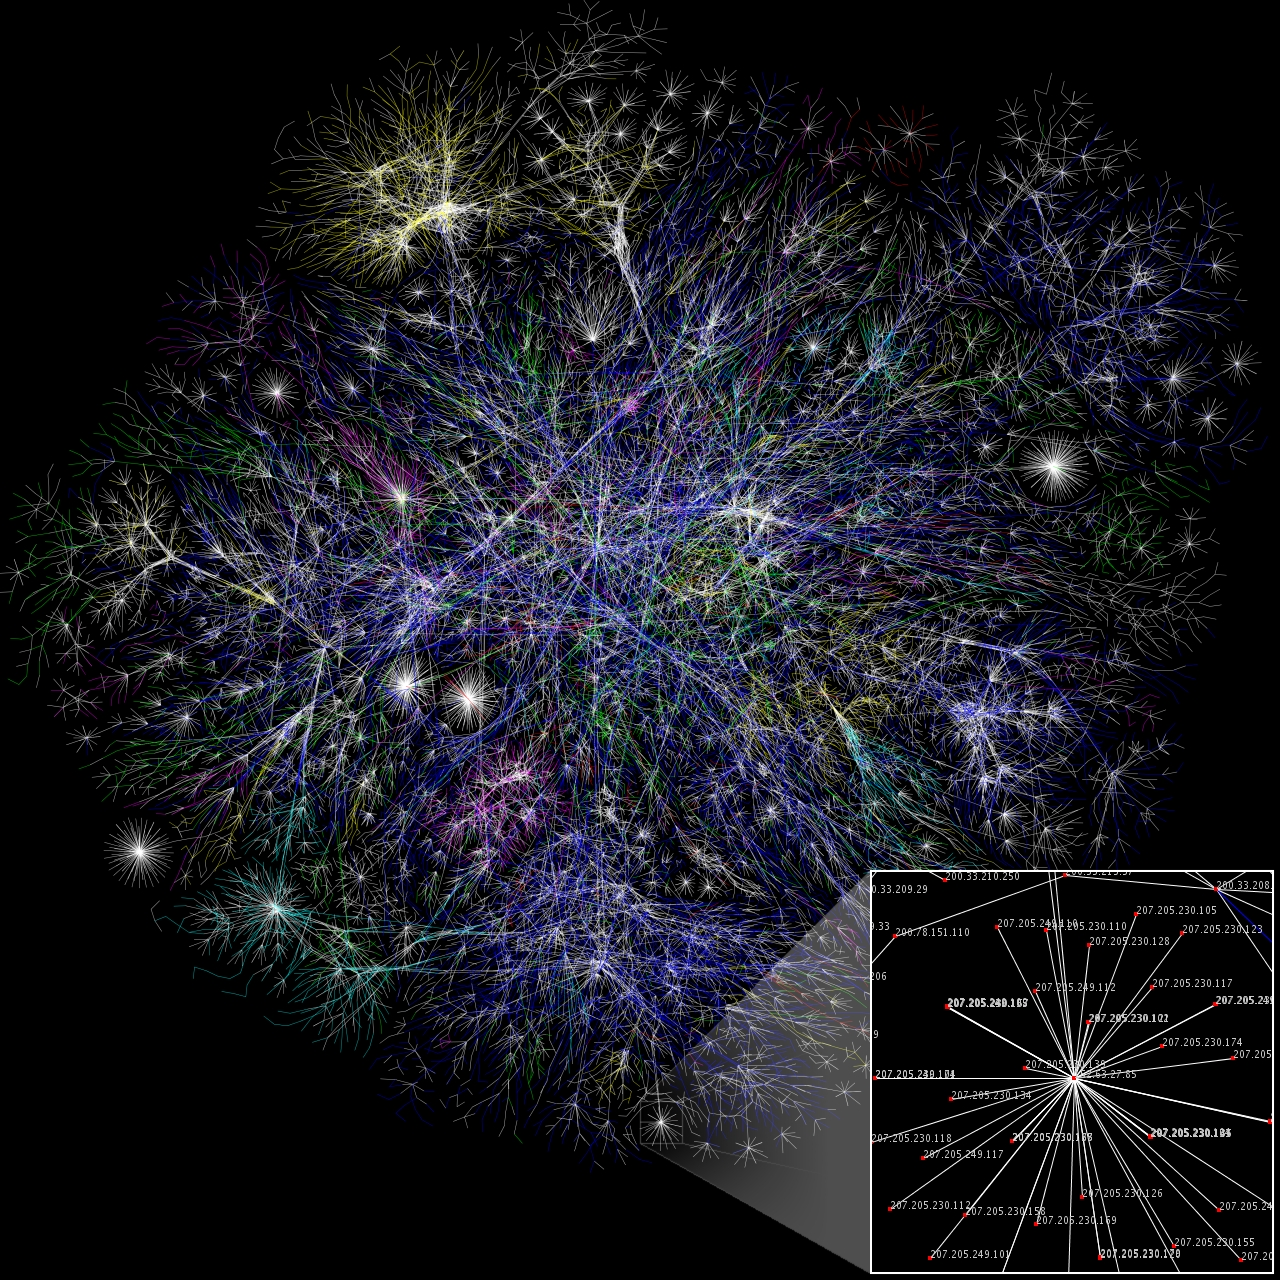
\includegraphics[width=\textwidth]{Internet_map_1024.jpg}
        \\
        {\small The Opte Project}

        \column{0.6\textwidth}
        Everyone seems to have data, and lots of it. Everyone seems to want pictures of their data.
    \end{columns}
\end{frame}

\begin{frame}{Cool Kids Do Data Visualization}
    \begin{columns}[c]
        \column{0.3\textwidth}
        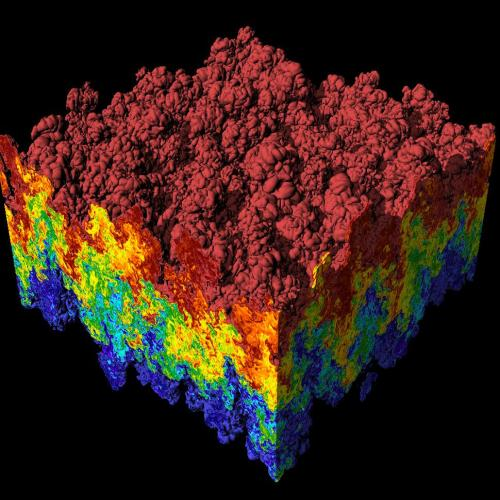
\includegraphics[width=\textwidth]{Rayleigh-Taylor_instability.jpg}
        \\
        {\small Lawrence Livermore National Laboratory}

        \column{0.6\textwidth}
        Visualization has become a vibrant field of study. People blog about visualizations.
    \end{columns}
\end{frame}

\begin{frame}{Cool Kids Do Data Visualization}
    In particular, people love geospatial visualization. Perhaps because
    everyone has geographic data, and Google's Maps API is easy.
    \begin{center}
        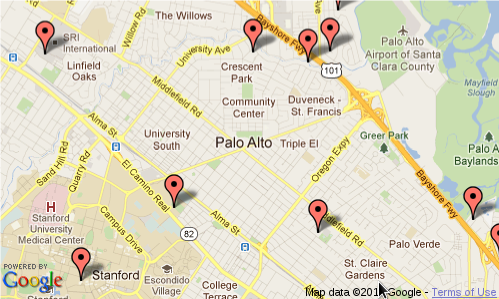
\includegraphics[width=0.8\textwidth]{Maps_API.png}
    \end{center}
\end{frame}

\begin{frame}{Cool Kids Do Data Visualization}
    \begin{center}
        ...or other APIs, if you prefer...
        \\
        \vspace{0.1\textheight}
        
\includegraphics[width=0.8\textwidth]{mapping_apis.png}
    \end{center}
\end{frame}

\begin{frame}{Geospatial Visualization}
    Geospatial visualization is \ldots
    \begin{itemize}
        \item It's easy to understand, compared to dots and lines. Everyone understands maps
        \item The selection of APIs makes it easy to do
        \item Everyone has geographic data
        \begin{itemize}
            \item Who browsed my website, from where? (GeoIP)
            \item Where do I ship most of my orders
            \item What, in fact, are the migration patterns of African and European swallows?
        \end{itemize}
    \end{itemize}
\end{frame}

\begin{frame}{Everyone has Geographic Data}
    \begin{varblock}[0.8\textwidth]{Note}
        Although everyone has geographic data, it's not necessarily important data.
    \end{varblock}
\end{frame}

\begin{frame}{Everyone has Geographic Data}
    \begin{varblock}[0.8\textwidth]{Note}
        The fact that data are unimportant rarely prevents people from trying to make a graph of it.
    \end{varblock}
\end{frame}

\begin{frame}{Google Earth}
    Google Earth is essentially Google Maps in 3D.
    \begin{center}
        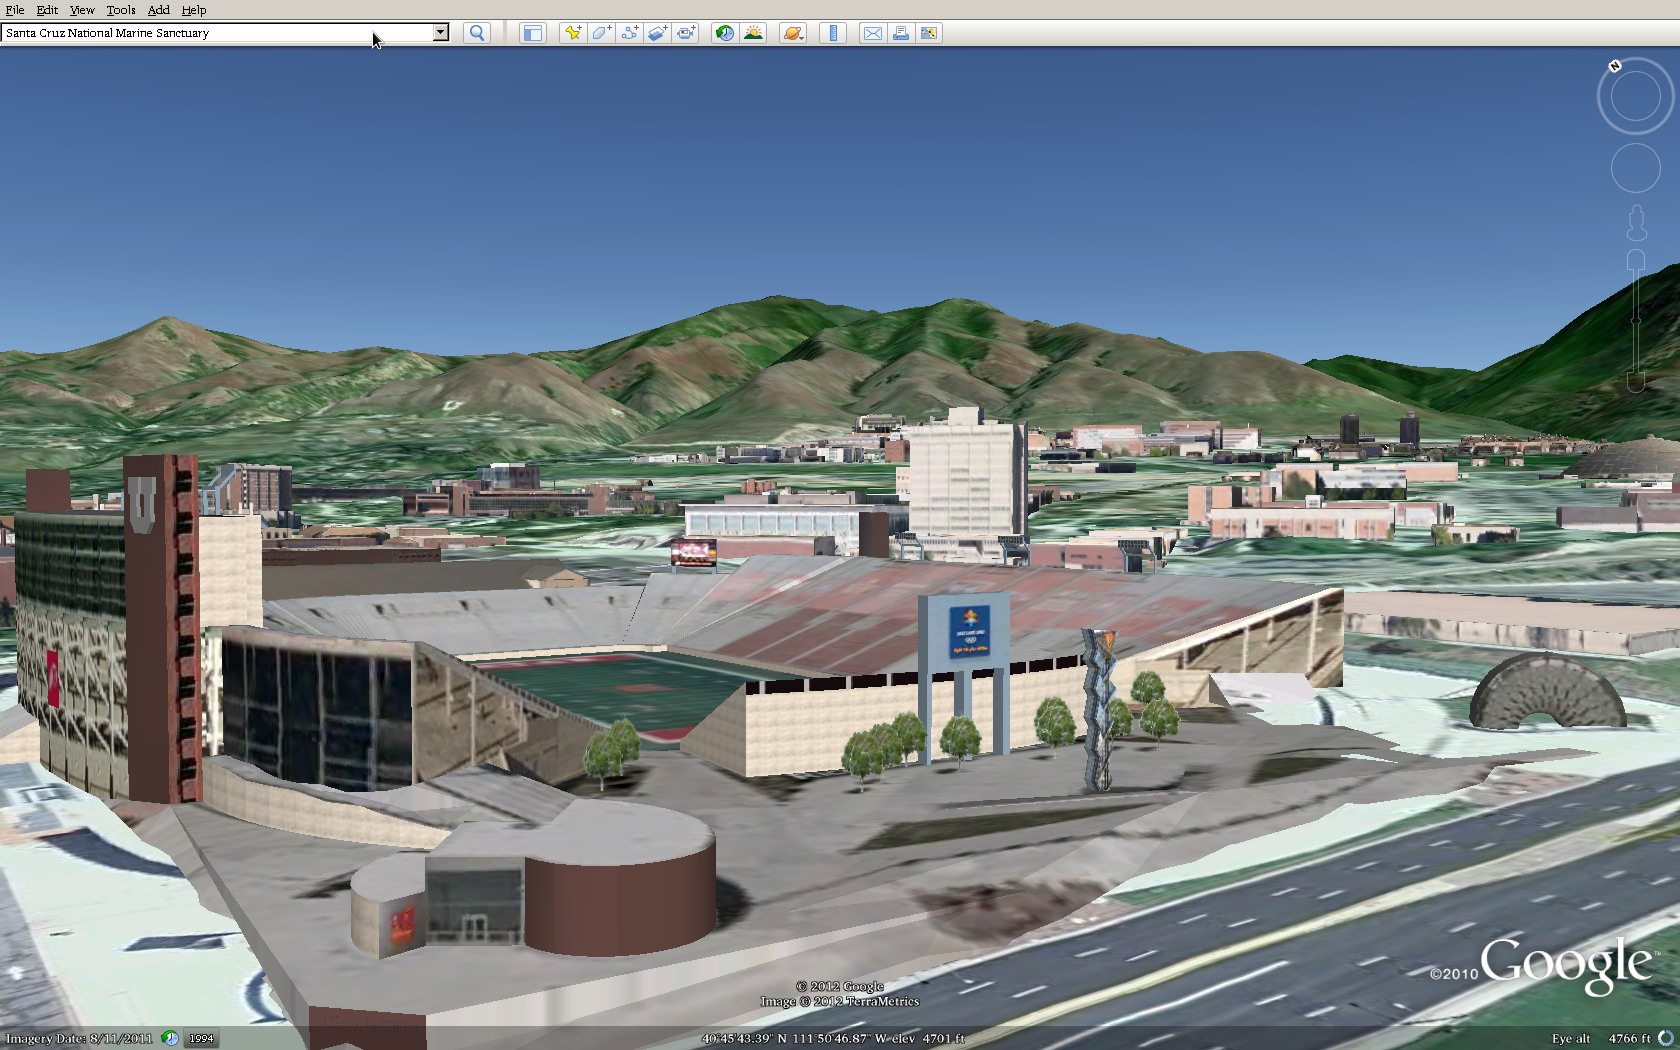
\includegraphics[width=0.8\textwidth]{RiceEcclesStadium.png}
    \end{center}
\end{frame}

%Having said all that, geospatial visualization continues to improve, and here
%we're going to talk about one way it has done so, namely with Google Earth.
%Google Earth takes Google Maps and makes it three dimensional. Users can
%manipulate a 3D model of the globe, zooming in and out and examining bits of
%the earth to their heart's content.  More importantly, Google Earth also lets
%users add various objects to the globe using an XML-based language called
%Keyhole Markup Language, or KML, after the Keyhole Corporation that developed
%the technology and got bought by Google in 2004.
%
%Here are some examples:
%
%<blah />
%
%So in order to give you some idea of what you can do with this stuff, let's
%cover some of the elements of KML. I'll avoid showing you lots of KML syntax,
%but rather just give you examples of KML objects as Google Earth displays them.
%Interested parties can review the reference documentation.
%
%Point
%
%The basic element in most everything is a point. Points have a latitude, a longitude, an altitude, and an altitude mode
%% XXX stopped at the line above
%Placemark
%Polygons (in limited detail)
%AbstractViews
%TimePrimitives
%Tours -- Flyto, AnimatedUpdate
%Regions
%
%One of Earth's neater features is its ability to synchronize itself with other
%instances of Earth. Linux media geeks may already be familiar with mplayer's
%similar functionality, which allows you to have one mplayer instance acting as
%master, and broadcasting timing information to one or more slave instances,
%which is useful for things like monitor walls.

\end{document}
